\documentclass[11pt,a4paper]{tesis}

\usepackage{graphicx}
\usepackage[utf8]{inputenc}
\usepackage[spanish]{babel}
\usepackage[left=3cm,right=3cm,bottom=3.5cm,top=3.5cm]{geometry}
\usepackage{amssymb}
\usepackage{float}
\usepackage{titlesec}
\usepackage{pdfpages}

\titleformat*{\subsubsection}{\large\bfseries}

\begin{document}

\def\titulo{Licenciado }
\def\autor{Ivan Pasquini}
\def\tituloTesis{Localización y modelado simultáneos \mbox{mediante} generación y actualización \mbox{automática} de controladores discretos}
\def\runtitulo{Localización y modelado simultáneos mediante generación y actualización automática de controladores discretos}
\def\runtitle{Localización y modelado simultáneos mediante generación y actualización automática de controladores discretos}
\def\director{Nicolás Roque D'Ippolito}
\def\codirector{Leandro Ezequiel Nahabedian}
\def\lugar{Buenos Aires, 2016}
\newcommand{\HRule}{\rule{\linewidth}{0.2mm}}
%
\thispagestyle{empty}

\begin{center}\leavevmode

\vspace{-2cm}

\begin{tabular}{l}

\includegraphics[width=2.6cm]{logofcen.pdf}
\end{tabular}


{\large \sc Universidad de Buenos Aires

Facultad de Ciencias Exactas y Naturales

Departamento de Computaci\'on}

\vspace{6.0cm}

%\vspace{3.0cm}
%{
%\Large \color{red}
%\begin{tabular}{|p{2cm}cp{2cm}|}
%\hline
%& Pre-Final Version: \today &\\
%\hline
%\end{tabular}
%}
%\vspace{2.5cm}

{\huge\bf \tituloTesis}

\vspace{2cm}

{\large Tesis presentada para optar al t\'{\i}tulo de\\
\titulo en Ciencias de la Computaci\'on}

\vspace{2cm}

{\Large \autor}

{LU: 141/09}

\end{center}

\vfill

{\large

{Director: \director}

\vspace{.2cm}


\lugar
}

\newpage\thispagestyle{empty}


\frontmatter
\pagestyle{empty}
%\begin{center}
%\large \bf \runtitulo
%\end{center}
%\vspace{1cm}
\chapter*{\runtitulo}

\noindent
En el área de robótica, el problema de la exploración consiste en recorrer, mediante un vehículo autónomo,
una zona desconocida para obtener conocimiento sobre ella. La utilización de robots es muy importante para
la cartografía o búsqueda y rescate en lugares que son peligrosos o inaccesibles para las personas.\\
En el caso de la utilización de robots autónomos, se utiliza la técnica de localización y modelado simultáneos, 
para construir un mapa de la zona desconocida en la que se encuentra el robot, a la vez que estima su 
trayectoria al desplazarse dentro de la misma.

\vspace{\baselineskip}
El objetivo de esta tesis es resolver el problema de localización y modelado simultáneos utilizando como modelo 
matemático los MTS (Modal Transition System), que son nociones abstractas de los LTSs (Labelled Transition Systems).\\
Dado conjunto de objetivos y un conjunto de suposiciones de dominio, los MTSs nos permiten determinar, mediante la 
síntesis de controladores, si los objetivos son imposibles de realizar, si podemos garantizar su cumplimiento, o si 
las suposiciones de dominio son insuficientes para decidir sobre los objetivos.

\vspace{\baselineskip}
Para cumplir con el objetivo de la tesis, extenderemos la herramienta MTSA (Modal Transition System Analyser) para
dar soporte a la exploración, y presentaremos una estrategia, que bajo ciertas condiciones, nos permita ir agregando 
información a nuestras suposiciones de dominio, hasta poder decidir si es o no posible garantizar el cumplimiento de
los objetivos de la exploración.

\bigskip

\noindent\textbf{Palabras claves:} Exploración, Modelado, LTS, MTS, Síntesis de controladores.

\clearpage
\chapter*{Agradecimientos}

\noindent
A mi familia, sin su soporte incondicional no me hubiera sido posible llegar a este punto.\\ 
A mis amigos, quienes me acompañaron durante todos estos años de carrera.


\noindent A mi director de tesis y colaboradores, Leandro Nahabedian, Nicolás 
D'Ippolito 
y Natalia Rodriguez, por su guía, consejo y tiempo.

\noindent Al jurado, por haberse dedicado a la lectura y corrección de esta 
tesis.

\cleardoublepage
\hfill \textit{A mi familia}

\clearpage
\tableofcontents

\mainmatter
\pagestyle{headings}

\chapter{Introducción}

\section{Motivación}

En el área de robótica, el problema de la exploración consiste en recorrer, mediante un robot autónomo, una zona 
desconocida para obtener el conocimiento total de esta, o en caso de no poder reconocerla en su totalidad, maximizar 
el espacio explorado. 


La utilización de robots es muy importante para la cartografía o búsqueda y rescate en lugares que son peligrosos o 
inaccesibles para las personas. Hay muchos ejemplos de exploración con robots autónomos, como las sondas espaciales 
no tripuladas que exploran lugares antes de que lleguen los astronautas, o robots que ingresan en estructuras colapsadas 
para crear una reconstrucción del entorno y reconocer exactamente el lugar en el que se encuentran las víctimas.


Los robots autónomos necesitan un mapa para poder operar en un entorno particular. Por esta razón, se utiliza la técnica 
de localización y modelado simultáneos, para construir un mapa de una zona desconocida en la que se encuentra el robot, 
a la vez que estima su trayectoria al desplazarse dentro de la misma.


Existen trabajos previos que logran generar un mapa mediante exploración, trabajando sobre entornos estáticos. 
Se utilizan diversas técnicas para el aprendizaje sobre el entorno, como por ejemplo redes neuronales \cite{TP2}, 
grafos \cite{TP4} o múltiples robots \cite{TP5}. Algunos trabajos dejan abierta la pregunta sobre como explorar 
entornos dinámicos \cite{TP1} \cite{TP3}. También existen trabajos previos que contemplan cambios en el entorno \cite{TP6}.


En este trabajo estamos interesados en decidir si es posible alcanzar un 
objetivo (posición) en el mapa evitando lo maximo posible que el robot explore 
la totalidad del mapa. 
Dicho problema fue explorado 
en~\cite{melchior2007particle} ampliando el algoritmo tradicional que otorga 
un camino hacia el objetivo para que soporte incertidumbre del area a recorrer. 

\section{Resumen de la contribución}

Las contribuciones de esta tesis pueden verse desde un punto de vista teórico. 
Durante los últimos años, para resolver problemas de alcanzabilidad de un 
objetivo en una area, se han usado algoritmos basados en camino mínimo como 
Dijkstra, A*, entre otros. Sin embargo, este trabajo queda como evidencia de 
que nuevas estrategias pueden usarse. Decidimos utilizar algoritmos de síntesis 
de controladores para poder resolver el problema descrito.

Por otro lado, las técnicas existentes de síntesis de controladores nos 
permiten hallar una estrategia para el robot cuando el area a transitar es 
totalmente conocida. Para casos donde esta suposición del ambiente es muy 
fuerte, actualmente, no existe forma de obtener un plan adecuado. La forma 
natural de modelar un area parcialmente conocida es mediante el modelado de un 
MTS (Modal Transition System), formalismo matemático que introduciremos en la 
sección~\ref{sec:MTS}. 

Previo a nuestro trabajo, la síntesis de controladores para dichos ambientes 
genera una respuesta trivaluada: ``Sin importar cómo se resuelvan las 
incertidumbre del ambiente, SIEMPRE obtendremos un plan para llegar al 
objetivo'', ``Sin importar cómo se resuelvan las incertidumbres del ambiente, 
NUNCA obtendremos un plan para llegar al objetivo'' o ``depende de cómo se 
resuelvan las incertidumbres''. Como contribución, extenderemos esta respuesta 
para que, en los casos favorables, además de asegurarnos la existencia, nos de 
el plan para llegar al objetivo.

En resumen, lo que queremos es poder dar una respuesta certera a si es posible 
garantizar 
el cumplimiento del objetivo. 
Para lograrlo necesitamos explorar para adquirir nueva información en caso de 
que la información que poseemos no sea 
suficiente para dar una respuesta. Extenderemos la herramienta MTSA (Modal 
Transition System Analyser) para dar soporte 
a la exploración y presentaremos una estrategia que nos permita dar una 
respuesta certera sobre la posibilidad de 
cumplimiento del objetivo.


\section{Esquema de la tesis}

A continuación, en el capítulo 2, introduciremos la teoría sobre la cual se 
sustenta nuestra 
solución al problema. 
En este capítulo definiremos formalmente la matemática necesarias que 
posteriormente vamos a utilizar. Luego, en el capítulo 3, introduciremos, 
formalmente, el problema a resolver. Presentaremos un algoritmo que lo resuelve 
y una posible estrategia de exploración que garantice encontrar una respuesta a 
este problema. El capítulo 4 muestra resultados de nuestra técnica.
Para ello, mostraremos como se comporta nuestro algoritmo y nuestra estrategia 
frente a una serie de problemas que servirán para mostrar las características 
de nuestra implementación. Despues en el capítulo 5, daremos conclusiones de 
este trabajo. Analizaremos el algoritmo y la estrategia, y plantearemos que 
trabajos a futuro podrían hacerse a partir de esta tesis. 
Finalmente, en el capítulo 6 y a modo de apendice, adjuntamos el manual de 
usuario para exploración en la herramienta MTSA basado en un ejemplo.


\chapter{Síntesis de controladores en entornos parcialmente conocidos}

Nuestro problema consiste en dado una posición inicial del sistema y un punto 
fisico objetivo dentro de una area/habitación, es requerido transladarnos al 
punto deseado. La particularidad de el problema a resolver es la falta de 
información que tenemos sobre el area donde transitar. Diremos entonces que 
buscaremos soluciones al problema de navegación de robots cuando el entorno es 
parcialmente conocido.
Tenemos un objetivo, pero no sabemos lo suficiente sobre el entorno como para 
decidir si es 
posible satisfacerlo. Debemos obtener el conocimiento necesario sobre el 
entorno para poder decidir sobre el objetivo. 
Por otro lado, el entorno puede ser tanto estático como dinámico. Será dinámico 
en caso de que mientras el robot intenta santisfacer su objetivo, existan 
componentes externos cuyas acciones modifican la configuración inicial del area 
a explorar.
Para lograrlo, vamos a utilizar los sensores del robot, los cuales nos aportan 
información, y una estrategia que 
utilice el conocimiento adquirido para obtener conocimiento nuevo.

Cuando comenzamos la exploración, la información que tenemos sobre el mundo es 
parcial. Los MTSs nos permiten codificar
la incertidumbre, ya que podemos distinguir la información que poseemos como 
transiciones requeridas y la información
que podemos adquirir mediante exploración como transiciones posibles. El mundo 
real, el cual estamos explorando, puede 
representarse como un LTS (Labelled Transition System) que refina nuestro MTS 
inicial.

Además del LTS que representa al mundo real, otros LTSs pueden refinar al MTS 
que representa nuestro conocimiento. Estos
LTSs representan a todas las posibles formas que puede llegar a tener el mundo 
real a partir del conocimiento que poseemos
actualmente. En cada uno de estos LTSs, las acciones posibles o bien van a ser 
acciones requeridas, o bien no van a formar
parte del LTS, y en caso de que sean acciones requeridas, puede variar la 
cantidad de veces que puede ejecutarse dicha acción.
Por estas razones, la cantidad de LTSs que refinan a nuestro MTS puede llegar a 
ser infinita. Cada uno de estos LTSs está
decidiendo sobre la incertidumbre del MTS que representa nuestro conocimiento 
actual.

Cuando exploramos, lo hacemos para poder realizar un objetivo. Mediante la 
síntesis de controladores, podemos intentar 
generar automáticamente una máquina, tal que al componerla en paralelo con el 
MTS que representa nuestro conocimiento 
del mundo, garantice el cumplimiento del objetivo.

Si para cada uno de los LTSs que refinan a nuestro MTS, el objetivo es 
alcanzable, sabemos que podemos garantizar el
cumplimiento del objetivo, ya que el mundo puede representarse como un LTS que 
refina nuestro modelo. Cuando no es posible
sintetizar un controlador que pueda garantizar que los objetivos se alcancen 
para ninguno de los LTSs que refinan a nuestro
modelo, podemos afirmar que el objetivo no es realizable en el mundo real. Pero 
si para algunos de estos LTSs existe un
controlador, y para otros no, no podemos afirmar nada sobre nuestro objetivo.

\section{Problema}

Una posible solución al problema de la síntesis de controladores en entornos 
parcialmente conocidos es un LTS $x$ (ver sección~\ref{sec:LTS}) tal que 
$M$ $\parallel$ $x$ $\models$ $G$, en donde $M$ es el MTS (ver 
sección~\ref{sec:MTS}) que modela el entorno y $G$ es un fórmula en FLTL (ver 
sección~\ref{sec:FLTL}) que describe cual es el sector objetivo. 

El estado del arte en cuanto a síntesis de controladores sobre Modal Transition 
Systems, nos otorga una respuesta trivaluada como mostramos previamente en la 
sección~\ref{sec:MTS_control}. Sin embargo, actualmente no existe forma de 
obtener un LTS solución ($x$). Si bien una de nuestras contribuciones es 
generar automáticamente el LTS $x$, la complejidad de producir dicho output 
depende de la configuración inicial de nuestros inputs. 
Por lo tanto podemos detallar tres casos al momento inicial de la ejecución:

\begin{itemize}

\item
\textit{Es posible sintetizar el LTS $x$ para cualquier implementación de $M$.} 
En otras 
palabras, sabemos que para toda incertidumbre que se encuentre en el area, sin 
importar qué encontremos al explorar esa zona, tenemos una estrategia que nos 
lleva al punto objetivo.

\item
\textit{No es posible sintetizar el LTS $x$ para ninguna implementación de 
$M$.} Esto es que sin importar como se resuelvan las incertidumbres, el sistema 
nunca va a poder alcanzar el objetivo.

\item
\textit{Algunas implementaciones de $M$ ofrecen buenas garantías para 
satisfacer el 
objetivo pero otras no. }
Por lo tanto, no sabemos si es posible sintetizar un controlador para la implementación de $M$ que representa al mundo real, el cual no conocemos.

\end{itemize}

En los dos primeros escenarios tenemos una respuesta a nuestro problema. De estar en el tercer escenario, queremos poder sintetizar 
el controlador en caso de ser posible, o tener garantías de que es imposible sintetizar dicho controlador. Para lograr nuestro objetivo 
debemos agregar información a M, para poder reducir su cantidad de posibles implementaciones, y que, de esta forma, su síntesis caiga 
en uno de los dos primeros escenarios.

La exploración nos permite adquirir conocimiento, ya que al observar mediante los sensores del robot lugares del entorno en los cuales 
no habíamos estado, podemos despejar la incertidumbre en nuestro modelo del entorno, representado por M. Vamos a realizar la exploración 
mediante un algoritmo, el cual se basa en ciclos de adquisición de conocimiento. Si nuestra información sobre el entorno es insuficiente, 
movemos al robot para que pueda aprender algo nuevo. Repetimos el ciclo hasta poder dar una respuesta.

Más formalmente podemos definir el problema síntesis de controladores en entornos parcialmente conocidos de la siguiente manera:

\begin{definition}{(Síntesis de controladores en entornos parcialmente conocidos)}
Sea $G$ una fórmula en FLTL que representa los requerimientos del sistema y $M$ es un MTS que representa las suposiciones del dominio conocidas en el momento inicial. Resolver el problema de síntesis de controladores en entornos parcialmente conocidos es decidir si existe un LTS $x$ tal que $M' \| x \models G$ donde $M' \prec M$ que representa el conocimiento inicial del entorno más todo el conocimiento adquirido por la exploración.
\end{definition}

\section{Algoritmo}

\begin{figure}[H]
  \centering
    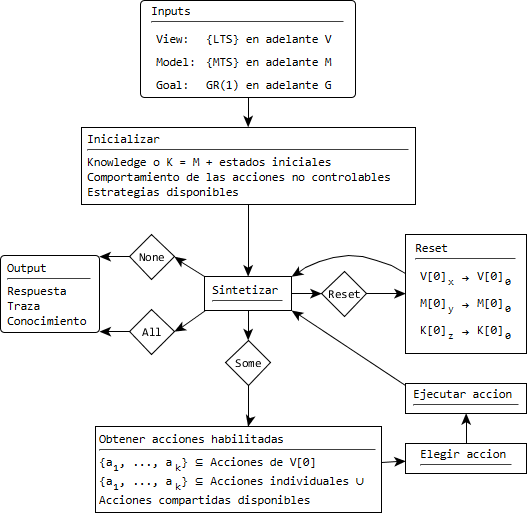
\includegraphics[scale=0.8]{Imagenes/Algoritmo/Algoritmo.png}
  \caption{Algoritmo de exploración.}
  \label{fig:Algoritmo}
\end{figure}

\begin{algorithm}
\begin{algorithmic}
\REQUIRE \{LTS\} View, \{MTS\} Model, GR(1) Goal
\ENSURE All si se puede satisfacer Goal en el Knowledge actual y None en caso contrario
\STATE Knowledge := Model $\cup$ estados iniciales
\STATE Respuesta := Sintetizar(Knowledge, Goal)
\WHILE {Respuesta == Some $||$ Respuesta == Reset}
\IF{Respuesta == Some}
\STATE Acciones habilitadas := \{a$_{1}$, ..., a$_{k}$\} tal que \{a$_{1}$, ..., a$_{k}$\} $\subseteq$ Acciones individuales(Knowledge[0]) $\cup$ Acciones compartidas disponibles(Knowledge[0])
\STATE Acción := Elegir(Knowledge, Acciones habilitadas)
\STATE Ejecutar(View, Model, Knowledge, Acciones controlables, Acción)
\ELSE
\STATE Reiniciar estados iniciales(View, Model, Knowledge)
\ENDIF
\STATE Respuesta := Sintetizar(Knowledge, Goal)
\ENDWHILE
\RETURN Respuesta
\end{algorithmic}
\caption{Algoritmo de exploración}
\end{algorithm}

\section{Inputs}

Para resolver el problema necesitamos poder observar al entorno a medida que nos movemos, saber con que información inicial 
contamos y tener un objetivo que cumplir.

\subsection{View}
\textbf{View} es una lista de LTSs. Representa el mundo sobre el cual se mueve el robot. 
El primer LTS de la lista representa el mapa del entorno, el cual regula como se mueve el robot por el mundo. Indica que acciones 
puede realizar en cada posición, y a que lugar lo llevan dichas acciones. 
Los otros LTSs representan el comportamiento de los agentes externos que interactúan con el entorno. Pueden bloquear y habilitar 
acciones en una determinada posición. El robot no tiene influencia sobre ellos. 
El robot solamente puede observar el estado actual del \textbf{View} mediante sus sensores. Sobre el mapa, solamente puede saber en qué posición 
está y que acciones puede ejecutar en dicha posición. Sobre los agentes externos, solamente puede observar su estado actual.

\subsection{Model}
\textbf{Model} es una lista de MTSs. Representa nuestro conocimiento inicial sobre el mundo. Por cada LTS en \textbf{View} hay un correspondiente MTS 
en \textbf{Model}. 
La única restricción para los MTSs de \textbf{Model}, es que puedan refinarse en sus correspondientes LTSs de \textbf{View}. Por lo tanto, como mínimo, 
cada MTS debe contar con un estado, y por cada acción en su correspondiente LTS, debe haber una acción posible en el MTS.

\subsection{Goal}
\textbf{Goal} es el objetivo del robot. Exploramos para poder decidir si es posible garantizar el cumplimiento de \textbf{Goal}. Está expresado con una 
fórmula GR\big(1\big).

\section{Inicialización}

\textbf{Knowledge} es una lista de MTSs que representa el conocimiento que vamos adquiriendo en cada iteración del algoritmo. En cada iteración, los MTSs 
de \textbf{Knowledge} son un refinamiento de los MTSs de la iteración anterior. Cada MTS de \textbf{Knowledge} se compone de dos grupos de estados: Los 
que están en \textit{La nube} y los que representan el conocimiento.


\textit{La nube} representa la incertidumbre. Es una copia del MTS de \textbf{Model}. Sus estados y acciones se mantienen inmutables en todas las 
iteraciones de \textbf{Knowledge}. 
El resto de los estados representan el conocimiento adquirido hasta el momento. Su cantidad de estados irá creciendo a medida que el robot adquiera información. 
En cada estado, las acciones que nunca fueron ejecutadas irán a un estado de 
\textit{La nube}, mientras que las que ya fueron ejecutadas, irán a un estado 
del conocimiento.


En la implementación del algoritmo en la herramienta MTSA, hay dos cuestiones importantes de inicialización. 
Por un lado, el comportamiento de las acciones no controlables de los agentes externos. Actualmente existen dos patrones de comportamiento. 
Por defecto, los agentes externos elegirán una acción al azar. El otro patrón de comportamiento consiste en que se comporten de forma cíclica ejecutando 
las acciones que nosotros pasamos como input. En el futuro podrá extenderse la herramienta con más patrones de comportamiento. 
La otra cuestión es la estrategia utilizada por el robot. En esta tesis presentamos una única estrategia que resuelve el problema, pero en el futuro puede 
extenderse la herramienta con estrategias diferentes.

\section{Síntesis}

\begin{figure}[H]
  \centering
    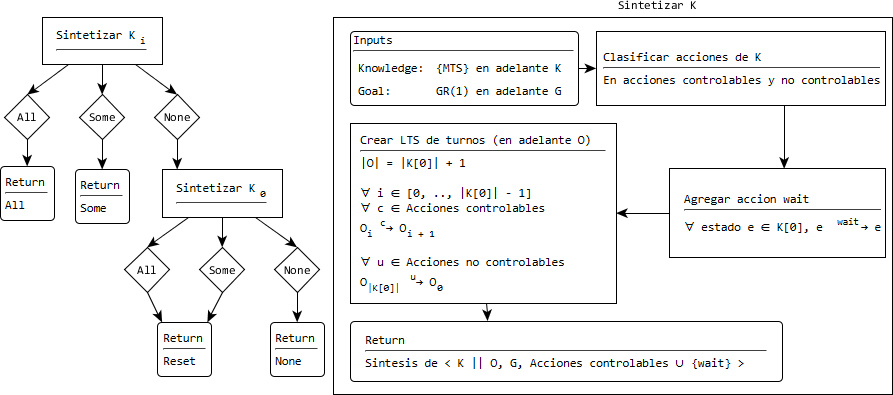
\includegraphics[width=1.0\textwidth]{Imagenes/Algoritmo/Algoritmo_sintetizar.png}
  \caption{Algoritmo de síntesis.}
  \label{fig:Algoritmo_sintetizar}
\end{figure}

\begin{algorithm}
\begin{algorithmic}
\REQUIRE \{MTS\} Knowledge, GR(1) Goal
\ENSURE Devuelve la respuesta al problema de control sobre Knowledge y Goal, o Reset si la respuesta es Some al volver la posición inicial de Knowledge al inicio
\STATE Knowledge en posición actual := Cambiar estado inicial a actual(Knowledge)
\STATE Respuesta := Problema de control(Knowledge en posición actual, Goal)
\IF{Respuesta == None}
\STATE Respuesta := Problema de control(Knowledge, Goal)
\IF{Respuesta == None}
\RETURN None
\ELSE
\RETURN Reset
\ENDIF
\ELSE
\RETURN Respuesta
\ENDIF
\end{algorithmic}
\caption{Algoritmo general de síntesis}
\end{algorithm}

\begin{algorithm}
\begin{algorithmic}
\REQUIRE \{MTS\} Knowledge, GR(1) Goal
\ENSURE La respuesta decide la realizabilidad de Goal sobre las implementaciónes de Knowledge
\STATE Acciones controlables := Obtener acciones controlables(Knowledge)
\STATE Acciones no controlables := Obtener acciones no controlables(Knowledge)
\FOR{Estado $\in$ Estados(Knowledge[0])}
	\STATE Agregar acción(Knowledge[0], WAIT, Estado, Estado)
\ENDFOR
\STATE LTS de turnos := Crear LTS de turnos(Knowledge, Acciones controlables, Acciones no controlables)
\STATE Respuesta := Síntesis(Knowledge $||$ LTS de turnos, Goal, Acciones controlables $\cup$ \{wait\})
\RETURN Respuesta
\end{algorithmic}
\caption{Algoritmo del problema de control sobre MTSs}
\end{algorithm}

\newpage

\subsection{Detalle}

Al principio de cada iteración, lo primero que hacemos es intentar dar una respuesta a la pregunta sobre si podemos garantizar el cumplimiento del objetivo. 
En otras palabras, queremos ver si podemos sintetizar un controlador que garantice el cumplimiento de \textbf{Goal}.

La síntesis la haremos sobre un MTS basado en \textbf{Knowledge}, pero con algunas modificaciones necesarias para modelar correctamente el problema. 
Primero cambiamos el estado inicial del primer MTS de \textbf{Knowledge}, el que representa el mapa, para que su estado inicial sea el estado en el que está 
situado actualmente el robot. Esto es para que el controlador garantice el objetivo desde nuestra posición actual.

Luego, al primer MTS de \textbf{Knowledge} (el mapa), le agregaremos en cada estado la acción controlable wait, que irá al mismo estado. 
Esto es para representar la posibilidad de que el robot espere en su posición actual un cambio en los agentes externos.

Por último, creamos un LTS de turnos que permita al robot moverse a cualquier estado antes de que los agentes externos realicen cambios. Esto es para evitar que los 
agentes externos esperen que el robot esté lejos para realizar una acción que beneficie al robot. El LTS de turnos permitirá que el robot se mueva una cantidad 
de veces igual a la cantidad de estados del primer MTS del \textbf{Knowledge} (el mapa) antes de que los agentes externos se muevan.

De esta forma, con la posibilidad de moverse y esperar en cualquier estado conocido, puede estar en el estado necesario para beneficiarse de las acciones de 
los agentes externos. Sintetizaremos el controlador para \textbf{Goal} sobre la composición en paralelo de los MTSs de \textbf{Knowledge}, incluyendo el MTS al 
cual le agregamos las acciones wait, con el LTS de turnos.

Si el resultado de la síntesis es que puede generarse un controlador para cualquier LTS que sea un refinamiento del MTS que armamos, significa que el robot 
puede cumplir el objetivo sin importar como sean las zonas inexploradas del entorno. El algoritmo termina, dando como resultado la garantía del cumplimiento 
de \textbf{Goal}.

En caso de que no pueda generarse un controlador mara ningún LTS que sea un refinamiento del MTS que armamos, hay que volver a realizar la síntesis, pero sin 
realizar el cambio del estado inicial. Si nuevamente no puede generarse un controlador, significa que es imposible cumplir \textbf{Goal}, sin importar como sean 
las zonas inexploradas del entorno, y el algoritmo termina confirmando la imposibilidad de cumplimiento de \textbf{Goal}. En caso contrario, significa que 
llegamos a un punto sin retorno, pero todavía hay zonas inexploradas que pueden ser alcanzadas desde el inicio, en las cuales podríamos o no cumplir el objetivo. 

En caso de que nuestro robot tenga la capacidad de volver al inicio, o utilizar otro robot desde la zona inicial, podemos seguir explorando cambiando los 
estados iniciales de los primeros componentes de \textbf{View}, \textbf{Model} y \textbf{Knowledge} (los que representan al mapa) al estado inicial del comienzo 
de la exploración. Al hacer esto contamos con la información recolectada hasta el momento, la cual puede utilizar la estrategia para no volver a caer en el 
punto sin retorno.

Por último, si la síntesis puede generar un controlador para algunas de las implementaciones del MTS que armamos, pero para otras no, significa que no tenemos 
suficiente información sobre el entorno como para decidir sobre el objetivo, y necesitamos seguir explorando para refinar el \textbf{Knowledge}.

\section{Estrategia}

En caso de que sea necesario seguir explorando, necesitamos que la estrategia decida la próxima acción a ejecutar. El algoritmo está preparado para que, 
al utilizar múltiples estrategias, detecte si alguna entra en un ciclo infinito y la reemplace por otra.

\begin{figure}[H]
  \centering
    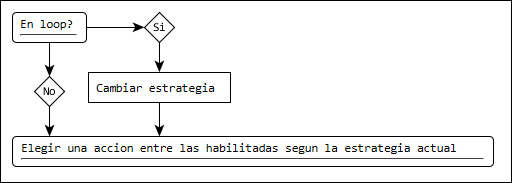
\includegraphics[scale=0.75]{Imagenes/Algoritmo/Algoritmo_elegir_1.png}
  \caption{Elección de estrategia}
  \label{fig:Algoritmo_elegir_1}
\end{figure}

\begin{algorithm}
\begin{algorithmic}
\REQUIRE \{MTS\} Knowledge, {Accion} Acciones habilitadas
\ENSURE Cambia la estrategia actual si entro en un ciclo
\IF{en un ciclo()}
\STATE Cambiar estrategia()
\ENDIF
\STATE Elegir(Knowledge, Acciones habilitadas)
\end{algorithmic}
\caption{Algoritmo de elección de estrategia}
\end{algorithm}


\subsection{Optimista}

Estamos por elegir una acción. Hacemos esto porque el intento de síntesis para generar un controlador que garantice \textbf{Goal} nos dio como resultado que 
existe un controlador para algunos refinamientos pero no para otros. En particular existe un controlador para el refinamiento más optimista, llamado 
controlador optimista. La estrategia Optimista aprovecha este hecho, ya que por construcción, el controlador optimista evitará las zonas inseguras. Lo que 
hace la estrategia es elegir de entre las acciones posibles, una acción que esté en el estado inicial del controlador optimista. En cambio, la estrategia 
Optimista - Nueva acción lo utiliza para filtrar de entre las acciones posibles, cuáles son las acciones seguras, y así elegir mediante la estrategia Nueva acción 
una acción entre las seguras.

\subsection{Nueva acción}

La estrategia Nueva acción tiene como objetivo ejecutar acciones nuevas, o en otras palabras, que no hayan sido ejecutadas anteriormente en su estado asociado. 
Si siempre ejecutamos acciones nuevas, siempre adquiriremos conocimiento nuevo, y como el entorno a explorar es finito, terminaremos por reconocerlo completamente 
de seguir esta estrategia.


La estrategia se divide en varias etapas. Lo primero que debemos hacer es saber sí, entre las acciones disponibles, existe alguna que no haya sido ejecutada 
anteriormente desde el estado actual. Si existe, la elegiremos, porque es una acción nueva.


Si el estado actual es un estado completamente explorado, o en otras palabras, ya ejecutamos anteriormente todas las acciones disponibles desde este estado, debemos 
llegar a un estado no completamente explorado. Para hacerlo, buscamos si hay algún estado que cumpla las condiciones deseadas al que podamos volver. Esto 
significa que exista un estado con alguna acción controlable como posible, y que podamos llegar a él por un camino de acciones requeridas en el primer componente 
de \textbf{Knowledge} (el mapa).


Para construir el camino, sintetizaremos un controlador con el objetivo de llegar a ese estado desde nuestro estado actual. Para lograrlo construiremos un MTS 
a partir del primer componente de \textbf{Knowledge}. Debemos agregar una acción ganadora al estado al que queremos llegar. El objetivo será ejecutar dicha acción, 
por lo cual para lograrlo tenemos que llegar al estado deseado desde nuestro estado actual. El segundo paso es eliminar las acciones posibles, para que el camino 
solo esté compuesto por acciones requeridas, o en otras palabras, ya ejecutadas anteriormente. En caso de existir el controlador buscado, necesitamos que el camino 
comience por alguna de las acciones disponibles desde nuestro estado actual. En este caso, la elegimos, porque nos acerca a una acción nueva.


Si no existen estados con acciones controlables no ejecutadas anteriormente, lo que tenemos que hacer es llegar a un estado con una acción compartida no ejecutada 
anteriormente, y esperar a que los agentes externos nos permitan ejecutarla. Seguimos el mismo procedimiento de síntesis utilizado anteriormente. Si existe el camino, 
elegimos la acción que nos permita acercarnos, en caso contrario eligiéremos esperar, ya que es necesaria la interacción de algún agente externo para poder continuar 
explorando.

\subsection{Optimista - Nueva acción}

En esta tesis vamos a presentar únicamente la estrategia Optimista - Nueva acción, la cual no entra en ciclos. Dicha estrategia es la composición de la estrategia 
Optimista, la cual busca evitar caer en zonas inseguras utilizando la información proporcionada por \textbf{Model}, y la estrategia Nueva acción, la cual busca siempre 
adquirir conocimiento nuevo utilizando información proporcionada por \textbf{Knowledge}.

\begin{figure}[H]
  \centering
    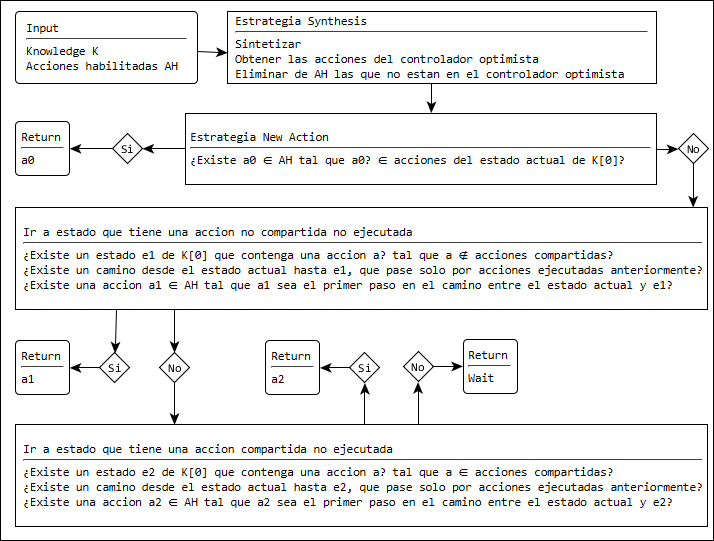
\includegraphics[scale=0.8]{Imagenes/Algoritmo/Algoritmo_elegir_2.png}
  \caption{Algoritmo de la estrategia Optimista - Nueva acción.}
  \label{fig:Algoritmo_elegir_2}
\end{figure}

\begin{algorithm}
\begin{algorithmic}
\REQUIRE MTS Knowledge, {Accion} Acciones habilitadas
\ENSURE Una accion que pertenece a Acciones habilitadas o Wait
\STATE Controlador optimista = Sintetizar(Knowledge)
\STATE Acciones del controlador optimista = obtener acciones habilitadas(Controlador optimista)
\STATE Acciones habilitadas = Acciones habilitadas $\cap$ Acciones del controlador optimista
\STATE Acciones habilitadas no ejecutadas = Acciones habilitadas $\cap$ acciones posibles(estado actual(Knowledge))
\IF{Acciones habilitadas no ejecutadas != $\emptyset$}
\RETURN Acciones habilitadas no ejecutadas[0]
\ELSE
\FOR{Estado $\in$ Estados(Knowledge)}
\IF{Estado == Estado inicial}
\STATE continue
\ENDIF
\STATE Acciones posibles no compartidas = acciones posibles no compartidas(Estado)
\IF{Acciones posibles no compartidas != $\emptyset$}
\STATE Controlador al estado = sintetizar para encontrar camino(Knowledge, Estado)
\STATE Acciones del controlador al estado = obtener acciones habilitadas(Controlador al estado)
\STATE Acciones habilitadas que llevan al estado = Acciones habilitadas $\cap$ Acciones del controlador al estado
\IF{Acciones habilitadas que llevan al estado != $\emptyset$}
\RETURN Acciones habilitadas que llevan al estado[0]
\ENDIF
\ENDIF
\ENDFOR
\FOR{Estado $\in$ Estados(Knowledge)}
\IF{Estado == Estado inicial}
\STATE continue
\ENDIF
\STATE Acciones posibles compartidas = acciones posibles compartidas(Estado)
\IF{Acciones posibles compartidas != $\emptyset$}
\STATE Controlador al estado = sintetizar para encontrar camino(Knowledge, Estado)
\STATE Acciones del controlador al estado = obtener acciones habilitadas(Controlador al estado)
\STATE Acciones habilitadas que llevan al estado = Acciones habilitadas $\cap$ Acciones del controlador al estado
\IF{Acciones habilitadas que llevan al estado != $\emptyset$}
\RETURN Acciones habilitadas que llevan al estado[0]
\ENDIF
\ENDIF
\ENDFOR
\RETURN Wait
\ENDIF
\end{algorithmic}
\caption{Algoritmo de la estrategia Optimista - Nueva acción}
\end{algorithm}

\newpage

\section{Ejecución}

\begin{figure}[H]
  \centering
    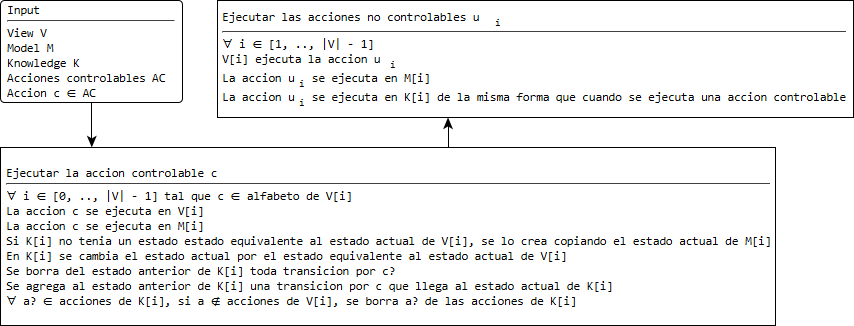
\includegraphics[width=1.0\textwidth]{Imagenes/Algoritmo/Algoritmo_ejecutar.png}
  \caption{Algoritmo de ejecución.}
  \label{fig:Algoritmo_ejecutar}
\end{figure}

\begin{algorithm}
\begin{algorithmic}
\REQUIRE \{LTS\} View, \{MTS\} Model, MTS Knowledge, {Accion} Acciones controlables, Accion Acción a ejecutar
\FOR{i = 0; i $<$ $|$View$|$; i++}
\IF{Acción a ejecutar $\notin$ Acciones(View[i])}
\STATE continue
\ENDIF
\STATE ejecutar(Accion acción a ejecutar, View[i])
\STATE ejecutar(Accion acción a ejecutar, Model[i])
\IF{Knowledge[i] == null}
\STATE Knowledge[i] = Model[i]
\ENDIF
\STATE Actualizar estado actual(Knowledge[i], View[i])
\STATE Eliminar transicion posible(Knowledge[i], Acción a ejecutar)
\STATE Agregar transicion(Knowledge[i], Acción a ejecutar)
\FOR{Accion posible in Acciones posibles(Knowledge[i])}
\IF{Accion posible $\notin$ Acciones posibles(View[i])}
\STATE Eliminar accion(Knowledge[i], Accion posible)
\ENDIF
\ENDFOR
\ENDFOR
\FOR{i = 1; i $<$ $|$View$|$; i++}
\STATE Ejecutar accion no controlable(View[i])
\STATE Ejecutar accion no controlable(Model[i])
\STATE Ejecutar accion no controlable(Knowledge[i])
\ENDFOR
\end{algorithmic}
\caption{Algoritmo de ejecución}
\end{algorithm}

Al ejecutar la acción elegida, el robot puede, o no, cambiar de ubicación en el entorno. Esto implica un cambio en el estado actual del primer componente tanto 
de \textbf{View}, como de \textbf{Model} y \textbf{Knowledge}. El primer componente de \textbf{Knowledge} también puede cambiar su estructura, refinando el MTS, 
como consecuencia de la nueva información aportada por los sensores del robot en su nueva ubicación.

Si es la primera vez que el robot se encuentra en la ubicación actual, se va a agregar un nuevo estado en el primer componente de \textbf{Knowledge}, en el que todas 
sus acciones se dirigen hacia \textit{La nube}. En caso de haber ejecutado una acción que se dirigía hacia \textit{La nube}, ahora podemos observar a que ubicación 
en el entorno nos lleva, por lo cual vamos a poder transformar en nuestro modelo dicha acción en una acción requerida que va hacia el estado correspondiente 
a la ubicación actual.

Luego de ejecutar la acción elegida, hay que ejecutar las acciones ejecutadas por los agentes externos. Los cambios en los agentes externos afectan el estado actual 
de las restantes componentes de \textbf{View}, \textbf{Model} y \textbf{Knowledge}, y la estructura de las restantes componentes de \textbf{Knowledge}. El proceso se 
realiza en la forma descripta por la figura 3.4.

\section{Ciclo de exploración}

\begin{figure}[H]
  \centering
    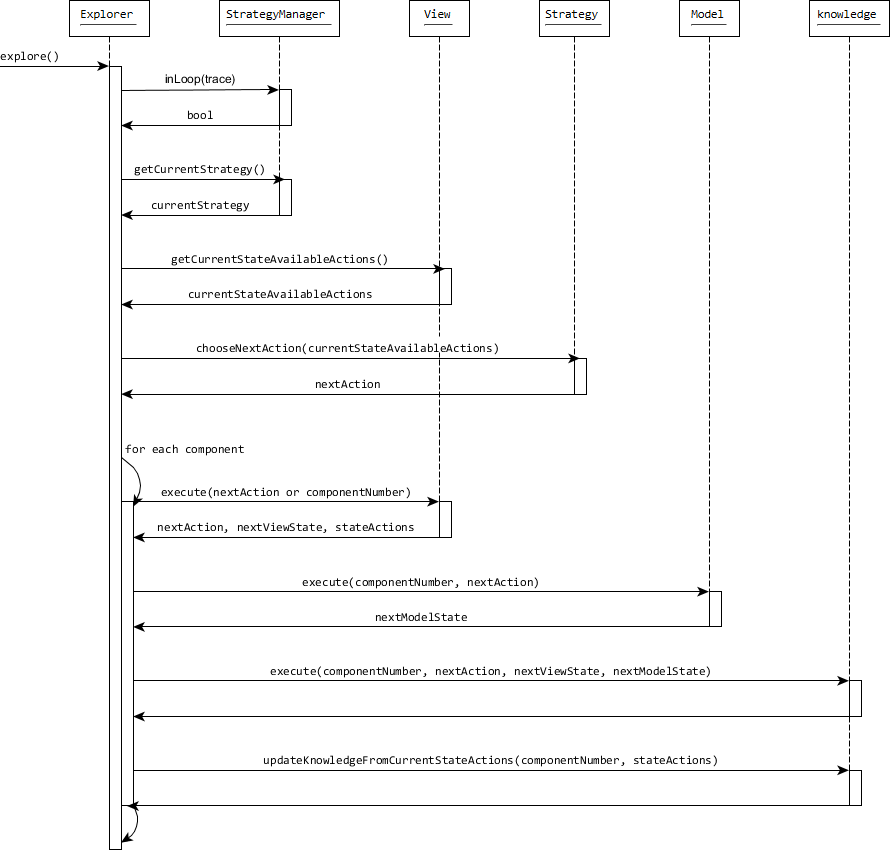
\includegraphics[width=1.0\textwidth]{Imagenes/Algoritmo/Secuencia_explorar.png}
  \caption{Diagrama de secuencia.}
  \label{fig:Secuencia_explorar}
\end{figure}

La figura 3.5 nos muestra cómo interactúan los diferentes objetos durante un ciclo de exploración.

Lo primero que hacemos es comprobar que la estrategia actual no haya entrado en un ciclo, ya que de no visitar estados nuevos no puede aportar información nueva.

En caso de que la estrategia actual esté en un ciclo la reemplazamos por otra. Una vez que tenemos la estrategia adecuada, observamos mediante los sensores que 
acciones tenemos disponibles en la ubicación actual, con el estado actual de los agentes externos. Le pedimos a la estrategia que elija una acción entre las 
acciones disponibles.

Cuando tenemos definida la siguiente acción, necesitamos ejecutarla. Primero la ejecutamos en \textbf{View}. Al hacerlo podemos censar en qué ubicación nos 
encontramos y qué acciones tenemos disponibles.

Luego la ejecutamos en \textbf{Model}, para que su estado actual se corresponda al estado que modela al estado actual de \textbf{View}.

A continuación, ejecutamos la acción en \textbf{Knowledge}, y en caso de que la acción vaya a un nuevo estado, utilizamos como nuevo estado el estado actual 
de \textbf{Model} (En este nuevo estado todas las acciones se dirigen hacia \textit{La nube}).

Por último, tenemos que agregar a \textbf{Knowledge} la nueva información obtenida, eliminando de su estado actual las acciones que no están disponibles, y 
transformando la acción que acabamos de ejecutar en caso de que originalmente estuviera dirigida hacia \textit{La nube}.

Luego de ejecutar la acción elegida, hay que ejecutar las acciones elegidas por los agentes externos. Cada componente extra en nuestros modelos representa a un agente 
externo, por lo tanto, hay que realizarlo una vez por componente. El proceso es el mismo que al ejecutar la acción elegida por nosotros, la única diferencia es que 
nosotros no elegimos la acción a ejecutar. Al hacer esto reflejamos el cambio en los agentes externos durante de tiempo que nos toma ejecutar nuestra acción.

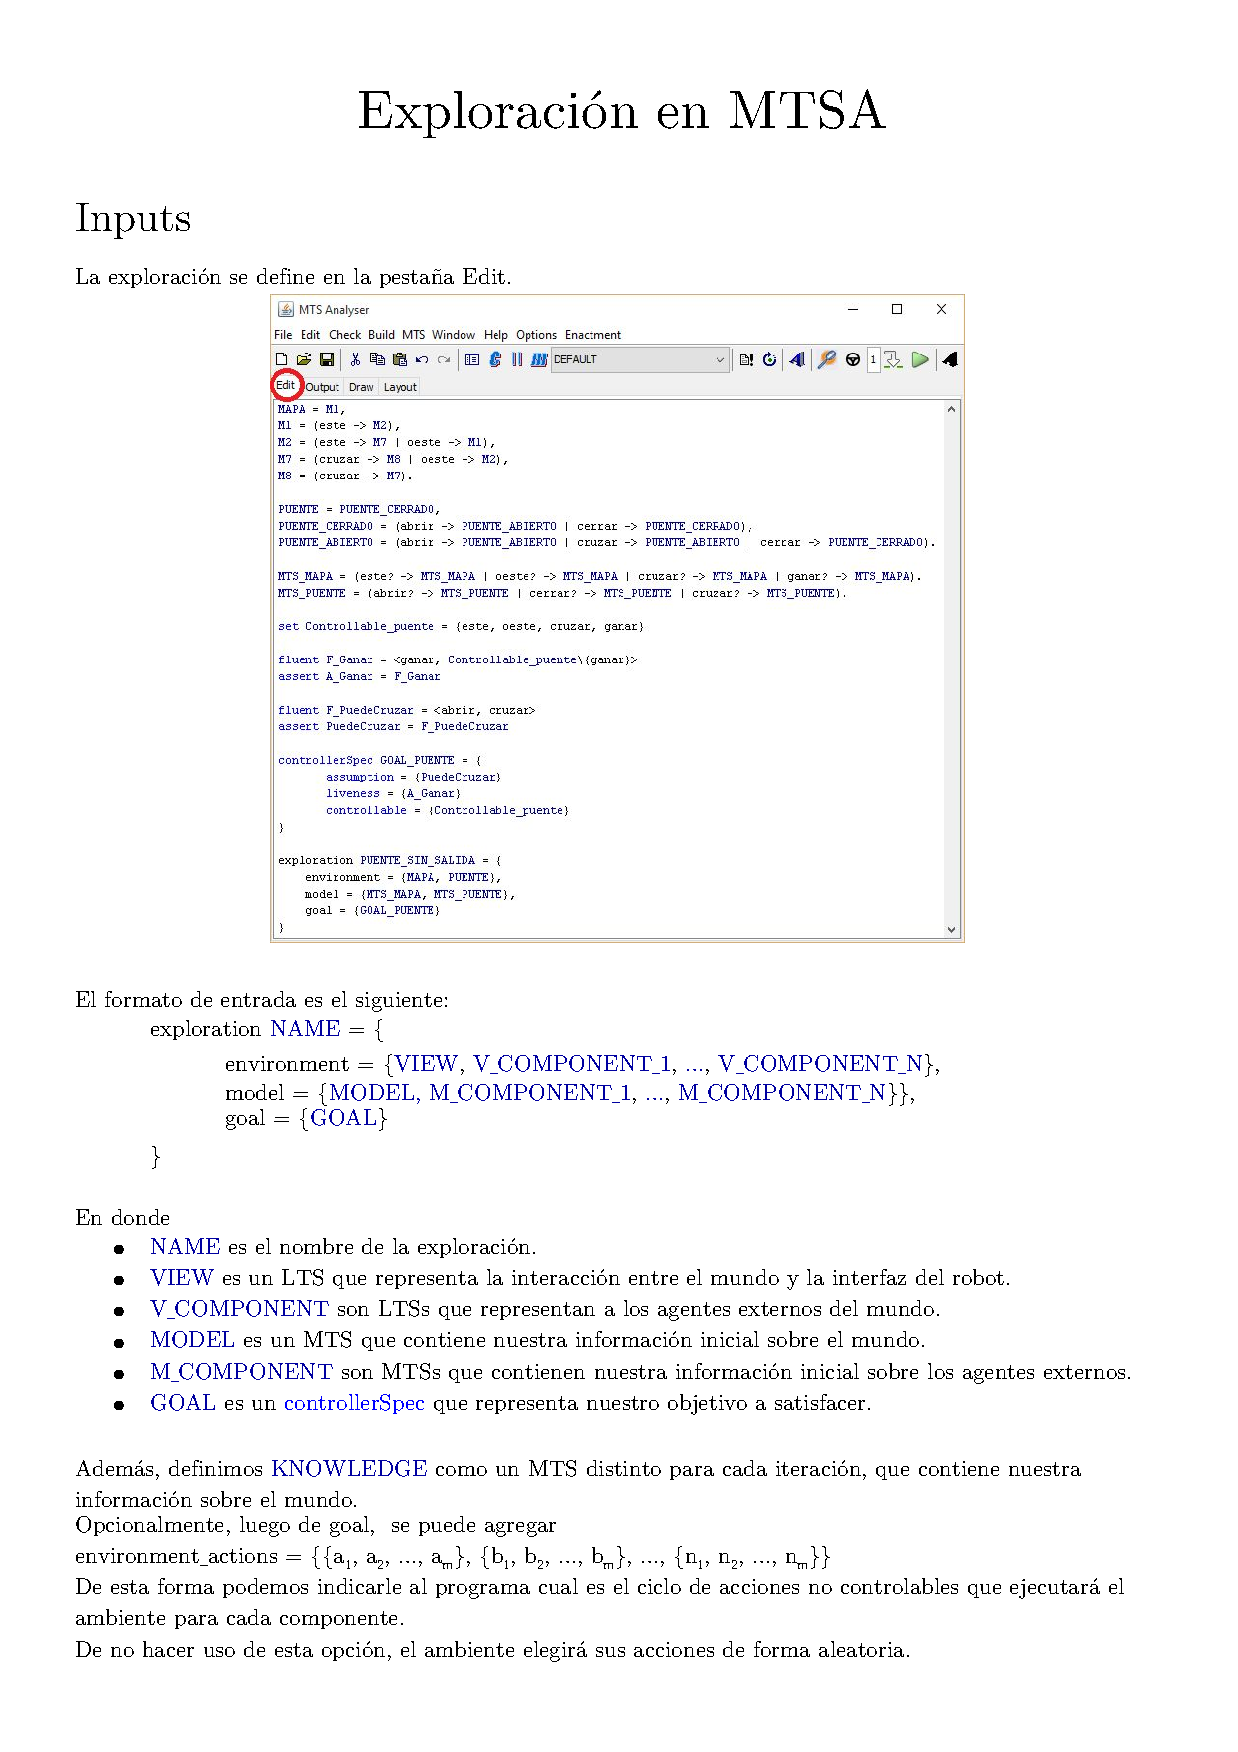
\includepdf[pages=-]{Manual.pdf}

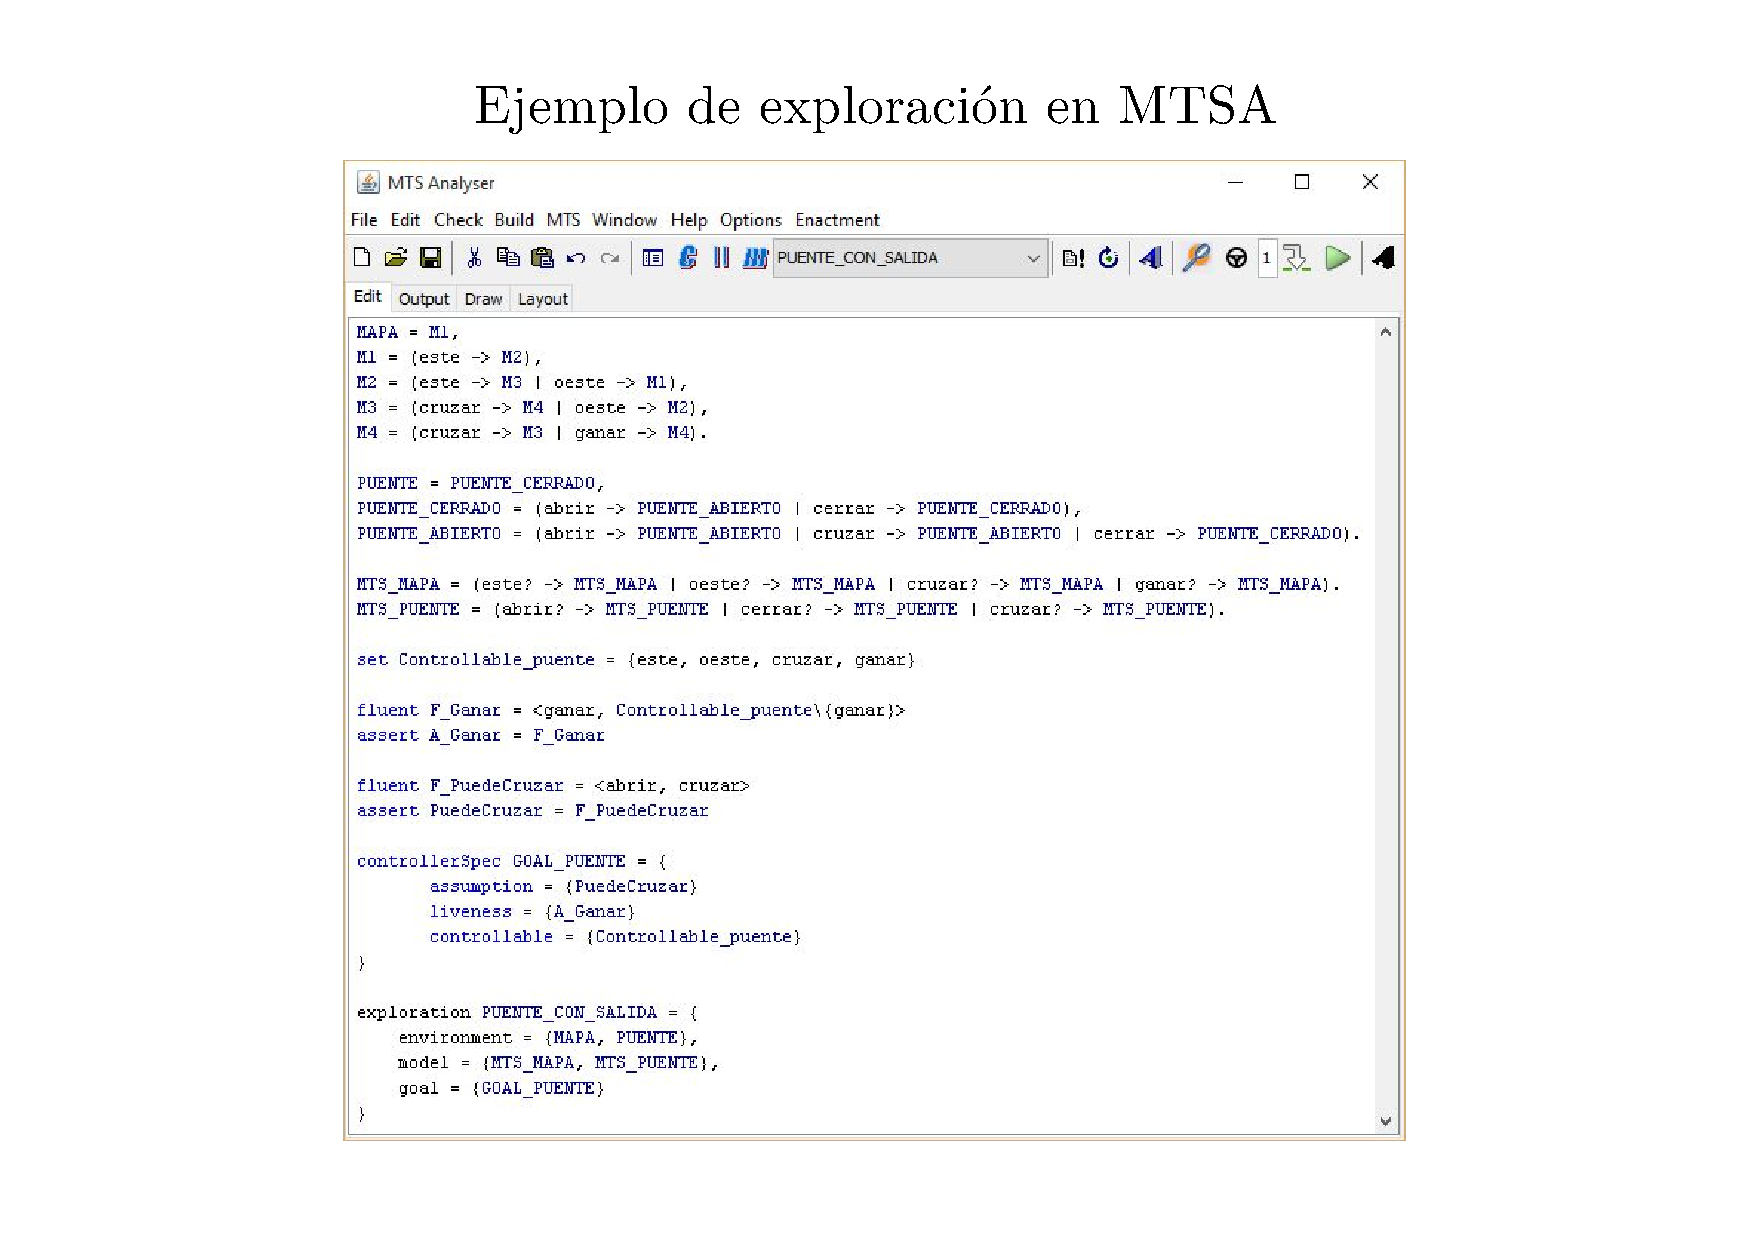
\includepdf[pages=-]{Ejemplo.pdf}

%%%% BIBLIOGRAFIA
\backmatter
%\bibliography{tesis}

\end{document}
